\documentclass[11pt]{article}
\usepackage[T1]{fontenc}
\usepackage[a4paper,margin=1in]{geometry}
\usepackage{graphicx}
\usepackage{tikz}
\usetikzlibrary{shapes.geometric,positioning,arrows.meta,calc,fit}
\usepackage{xcolor}
\usepackage{tabularx}
\usepackage{longtable}
\usepackage{booktabs}
\usepackage{array}
\usepackage{multirow}
\usepackage{colortbl}
\usepackage{enumitem}
\usepackage{titlesec}
\usepackage{fancyhdr}
\usepackage{hyperref}
\usepackage{parskip}
\hypersetup{colorlinks=true, linkcolor=black, urlcolor=blue, citecolor=black}

\titleformat{\section}{\Large\bfseries}{\thesection.}{0.5em}{}
\titleformat{\subsection}{\large\bfseries}{\thesubsection}{0.5em}{}
\titleformat{\subsubsection}{\normalsize\bfseries}{\thesubsubsection}{0.5em}{}

\pagestyle{fancy}
\fancyhf{}
\fancyfoot[C]{\thepage}
\renewcommand{\headrulewidth}{0pt}

\newcommand{\ucbox}[6]{%
  \noindent\rule{\linewidth}{0.5pt}\par
  \textbf{Use Case:} #1\par
  \textbf{Actor:} #2\par
  \textbf{Description:} #3\par
  \textbf{Preconditions:} #4\par
  \textbf{Postconditions:} #5\par
  \textbf{Main Flow:}\par
  #6
}

\begin{document}

% ================= TITLE PAGE =================
\begin{titlepage}
\centering
\vspace*{1.5cm}
{\Huge \textbf{PromptBench}}\\[0.6cm]
{\large \textbf{UCS 318 Software Engineering Project Report -- Semester Evaluation}}\\[1.2cm]

{\bf Submitted by:}\\[0.2cm]
Ridham Goyal (1024030417)\\[0.15cm]
Niloy Sharma (1024030422)\\[0.8cm]

{\bf Year: 2026--27 \quad|\quad Branch: COE}\\
{\bf Group: 3C31}\\[1cm]

{\bf Submitted to:}\\[0.2cm]
Hardik Sir\\[1.2cm]


\includegraphics[width=3.2cm]{images/thapar_logo.png}\\[0.8cm]

{\bf Computer Science and Engineering Department}\\
{\bf TIET, Patiala}\\
{\bf 2026}

\end{titlepage}

% ================= ACKNOWLEDGEMENT =================
\section*{Acknowledgement}
We take this opportunity to express our sincere gratitude to everyone who contributed to the
successful completion of our project ``PromptBench.''

First and foremost, we would like to extend our heartfelt thanks to Hardik Sir for
continuous guidance, valuable suggestions, and constructive feedback throughout the duration
of our project. Their encouragement and expertise played a pivotal role in helping us
understand the technical challenges and refine our approach at every stage.

We are also grateful to the Thapar Institute of Engineering and Technology (TIET) for
providing us with the necessary resources, infrastructure, and learning environment required
to develop this project effectively. Their support enabled us to explore, design, and build a
fully functioning system with confidence. Our sincere thanks also go to our peers and
classmates for their insightful discussions, suggestions, and motivation during the
development of this work. Lastly, we would like to express our deep appreciation to our
families for their constant encouragement, patience, and belief in us.

We wholeheartedly dedicate this project to everyone who supported us, guided us, and stood
by us in completing PromptBench successfully.

\vspace{0.5cm}
\begin{table}[h]
\centering
\begin{tabular}{|c|l|c|}
\hline
\textbf{S.No.} & \textbf{Student Name} & \textbf{Roll Number} \\
\hline
1 & Ridham Goyal & 1024030417 \\
\hline
2 & Niloy Sharma & 1024030422 \\
\hline
\end{tabular}
\end{table}

\newpage
\tableofcontents
\newpage

% ================= SECTION 1: PROJECT SELECTION PHASE =================
\section{Project Selection Phase}
In this phase, the final project idea is chosen based on feasibility, requirements, and expected
outcomes. This provides a clear foundation for preparing the software bid.

\subsection{Software Bid}

Please enter the names of your preferred team members:
\begin{itemize}[nosep]
  \item You are required to form a two to four person team.
  \item Choose your team members wisely. You will not be allowed to change teams.
\end{itemize}

\begin{longtable}{|p{2.6cm}|p{1.8cm}|p{4.3cm}|p{3cm}|p{1.5cm}|}
\hline
\textbf{Name} & \textbf{Roll No} & \textbf{Project Experience} & \textbf{Programming Language used} & \textbf{Signature} \\
\hline
Ridham Goyal & 1024030417 & [Describe relevant project experience] & [Languages used] & \\
\hline
Niloy Sharma & 1024030422 & [Describe relevant project experience] & [Languages used] & \\
\hline
\end{longtable}

\textbf{Programming Language / Environment Experience}\\
List the languages you are most comfortable developing in, as a team, in your order of
preference:
\begin{enumerate}[nosep]
  \item Python
  \item JavaScript
  \item [Add further languages]
\end{enumerate}

\textbf{Choices of Projects}

\begin{longtable}{|p{2cm}|p{3.5cm}|p{8.3cm}|}
\hline
 & \textbf{Project Name} & \textbf{Unique Selling Point} \\
\hline
First Choice & PromptBench &
Most coding-assessment platforms grade whether a candidate can write an algorithm.
PromptBench instead grades a skill that matters just as much on the job today: working
effectively with an AI assistant to solve an open-ended business problem. Candidates
investigate a case by chatting with a Helper AI, then submit a final recommendation that is
privately graded by a separate Judge AI against a hidden rubric and ground-truth notes --
without ever exposing the grading criteria to the Helper AI itself. \\
\hline
Second Choice & [Project name] & [Describe USP] \\
\hline
Third Choice & [Project name] & [Describe USP] \\
\hline
Fourth Choice & [Project name] & [Describe USP] \\
\hline
\end{longtable}

\textbf{Additional Remarks / Inputs}\\
The development of PromptBench provided valuable insight into designing systems where an
AI component must be trusted for one purpose (assisting) but explicitly distrusted for another
(grading). The backend -- authentication, case-study delivery, the Helper AI chat loop, the
Judge AI grading pipeline, and anti-gaming checks -- is complete and covered by an
end-to-end automated test suite. The React frontend is now also complete, with all planned
pages (login, signup, case list, case workspace, score dashboard, attempt history) wired to the
live backend. The main items remaining are deployment of the frontend and backend, and
expanding the seed content from 5 to the 8--10 case studies targeted for ``feature complete.''

\subsection{Project Overview}

\textbf{Purpose}\\
The main goal of PromptBench is to:
\begin{itemize}[nosep]
  \item Provide realistic, open-ended business case studies for practicing AI-assisted problem solving.
  \item Let a candidate work through a case with a conversational Helper AI before committing to an answer.
  \item Grade the candidate's process, not just their final answer, using a private Judge AI and a hidden rubric.
  \item Detect attempts to game the evaluation, such as submitting a pre-written answer with no real investigation.
\end{itemize}

\textbf{Target Users}
\begin{itemize}[nosep]
  \item \textbf{Candidates} -- register, attempt case studies, and review their scored history.
  \item \textbf{Helper AI} -- a scoped, candidate-facing assistant with access only to public case context.
  \item \textbf{Judge AI} -- a server-side evaluator invoked only at submission time.
\end{itemize}

\textbf{Key Features}
\begin{itemize}[nosep]
  \item Secure signup/login with JWT-protected sessions and bcrypt-hashed passwords.
  \item A library of business case studies spanning three categories: data diagnosis, strategy generation, and customer reasoning.
  \item A persisted chat workspace where every candidate message and Helper AI reply is stored as a transcript turn.
  \item A one-shot Judge AI grading call that returns a structured, rubric-based score with reasoning.
  \item Automated anti-gaming checks (near-zero conversation, too-fast submission, pre-written-answer detection).
  \item A personal history dashboard of past attempts and scores.
\end{itemize}

\textbf{System Overview}\\
PromptBench operates as a web-based platform where:
\begin{enumerate}[nosep]
  \item A candidate creates an account and logs in.
  \item The candidate browses the available business case studies.
  \item The candidate opens a Case Workspace, reviews the case context, and interacts with the Helper AI.
  \item The candidate drafts and submits a final recommendation.
  \item The Judge AI privately grades the full transcript and final answer against the hidden rubric and ground truth.
  \item The candidate reviews their overall score, per-dimension breakdown, and reasoning, and can revisit past attempts at any time.
\end{enumerate}

\newpage
% ================= SECTION 2: ANALYSIS PHASE =================
\section{Analysis Phase}

\subsection{Use Case}

\textbf{Actors}
\begin{itemize}[nosep]
  \item Candidate
  \item Helper AI (system actor)
  \item Judge AI (system actor)
\end{itemize}

\textbf{Candidate Use Cases}
\begin{enumerate}[nosep]
  \item Sign Up / Log In
  \item Browse Case Studies
  \item Start a Case Attempt
  \item Chat with Helper AI
  \item Draft and Submit Final Answer
  \item View Evaluation Score
  \item View Attempt History
\end{enumerate}

\textbf{System Actor Use Cases}
\begin{enumerate}[nosep,start=8]
  \item Generate Helper AI Response
  \item Run Anti-Gaming Checks
  \item Grade Submission
\end{enumerate}

\subsubsection{Use-Case Diagram}

The use-case diagram of the PromptBench system illustrates the interactions between the
Candidate and the two AI actors -- Helper AI and Judge AI -- and the system's functionalities.
A candidate can sign up, log in, browse case studies, start an attempt, chat with the Helper
AI, and submit a final answer. Submitting a final answer includes running anti-gaming checks
and invoking the Judge AI, which never interacts with the candidate directly. The Helper AI is
only ever invoked while a chat message is being sent, and never has access to the grading
path.

\begin{figure}[h]
\centering
\resizebox{\textwidth}{!}{%
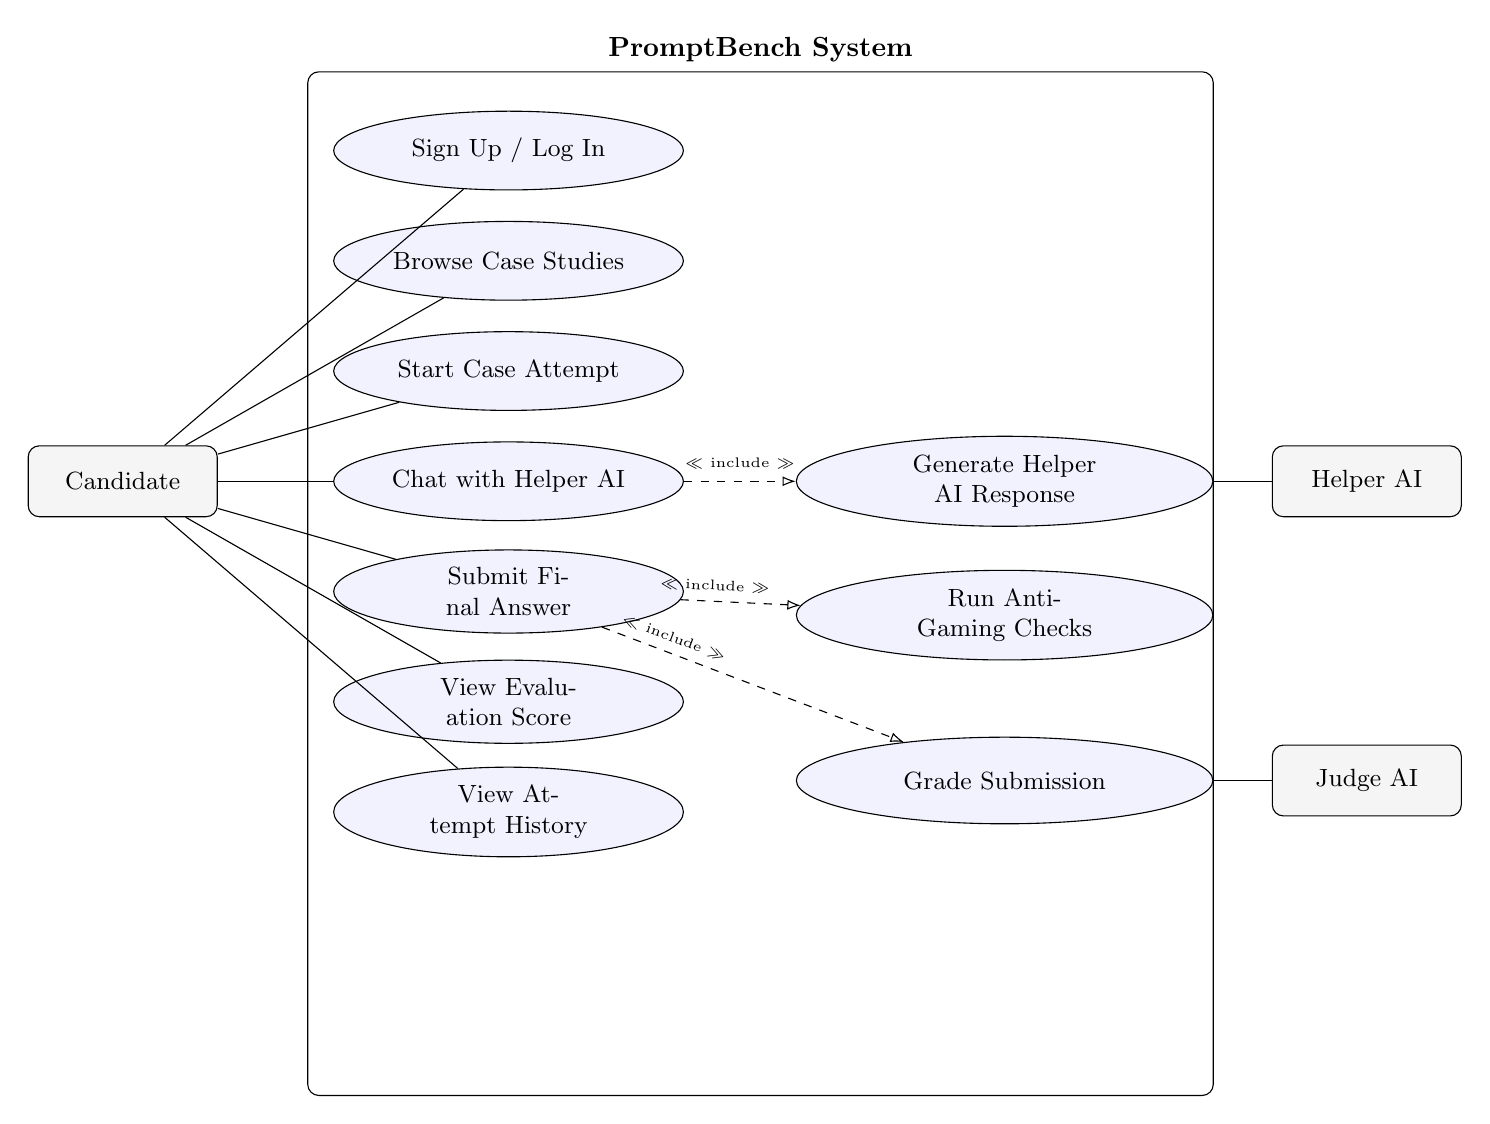
\begin{tikzpicture}[
  actor/.style={draw, rounded corners, fill=gray!8, minimum width=2.4cm, minimum height=0.9cm, align=center, font=\small},
  usecase/.style={draw, ellipse, fill=blue!5, text width=3cm, minimum height=1cm, align=center, font=\small, inner sep=2pt},
  wideusecase/.style={draw, ellipse, fill=blue!5, text width=3.6cm, minimum height=1.1cm, align=center, font=\small, inner sep=2pt},
  boundary/.style={draw, rounded corners, minimum width=11.5cm, minimum height=13cm}
]
  \node[boundary, label={[font=\bfseries]above:PromptBench System}] (sys) at (5.5,1.5) {};

  \node[usecase] (uc1) at (2.3,7) {Sign Up / Log In};
  \node[usecase] (uc2) at (2.3,5.6) {Browse Case Studies};
  \node[usecase] (uc3) at (2.3,4.2) {Start Case Attempt};
  \node[usecase] (uc4) at (2.3,2.8) {Chat with Helper AI};
  \node[usecase] (uc5) at (2.3,1.4) {Submit Final Answer};
  \node[usecase] (uc9) at (2.3,0.0) {View Evaluation Score};
  \node[usecase] (uc10) at (2.3,-1.4) {View Attempt History};

  \node[wideusecase] (uc6) at (8.6,2.8) {Generate Helper AI Response};
  \node[wideusecase] (uc7) at (8.6,1.1) {Run Anti-Gaming Checks};
  \node[wideusecase] (uc8) at (8.6,-1.0) {Grade Submission};

  \node[actor] (candidate) at (-2.6,2.8) {Candidate};
  \node[actor] (helper) at (13.2,2.8) {Helper AI};
  \node[actor] (judge) at (13.2,-1.0) {Judge AI};

  \draw (candidate) -- (uc1);
  \draw (candidate) -- (uc2);
  \draw (candidate) -- (uc3);
  \draw (candidate) -- (uc4);
  \draw (candidate) -- (uc5);
  \draw (candidate) -- (uc9);
  \draw (candidate) -- (uc10);

  \draw[dashed,-{Latex[open]}] (uc4) -- node[above,font=\tiny,yshift=1pt]{$\ll$ include $\gg$} (uc6);
  \draw[dashed,-{Latex[open]}] (uc5) -- node[above,font=\tiny,pos=0.28,sloped]{$\ll$ include $\gg$} (uc7);
  \draw[dashed,-{Latex[open]}] (uc5) -- node[above,font=\tiny,pos=0.22,sloped]{$\ll$ include $\gg$} (uc8);

  \draw (helper) -- (uc6);
  \draw (judge) -- (uc8);
\end{tikzpicture}%
}
\end{figure}

\newpage
\subsubsection{Use-Case Templates}

\ucbox{Sign Up / Log In}{Candidate}
{Candidate creates an account or authenticates to obtain a session token.}
{None}
{Candidate holds a valid JWT and can access protected routes.}
{
\begin{enumerate}[nosep]
  \item Candidate submits email, password (and name, if signing up).
  \item System validates credentials / uniqueness of email.
  \item System hashes and stores the password (signup) or verifies it (login).
  \item System issues a signed JWT on successful login.
\end{enumerate}
}

\vspace{0.3cm}
\ucbox{Browse Case Studies}{Candidate}
{Candidate views the list of available business case studies.}
{Candidate is authenticated.}
{List of case studies (title, category, difficulty) is displayed.}
{
\begin{enumerate}[nosep]
  \item Candidate opens the question list page.
  \item System fetches all questions from the database.
  \item System returns title, category, and difficulty for each case.
\end{enumerate}
}

\vspace{0.3cm}
\ucbox{Start Case Attempt}{Candidate}
{Candidate begins a new attempt on a chosen case study.}
{Case study exists.}
{A new submission record is created in the \texttt{in\_progress} state.}
{
\begin{enumerate}[nosep]
  \item Candidate selects a case study.
  \item System verifies the case exists.
  \item System creates a submission owned by the candidate.
\end{enumerate}
}
\textbf{Relationship:} Precedes $\rightarrow$ Chat with Helper AI

\vspace{0.3cm}
\ucbox{Chat with Helper AI}{Candidate}
{Candidate exchanges messages with the Helper AI while investigating the case.}
{Submission is in progress and owned by the candidate.}
{Candidate and assistant turns are persisted to the transcript.}
{
\begin{enumerate}[nosep]
  \item Candidate sends a message.
  \item System stores the candidate's turn.
  \item System calls the Helper AI with the public case context and full chat history.
  \item System stores the Helper AI's reply and returns it to the candidate.
\end{enumerate}
}
\textbf{Relationship:} Includes $\rightarrow$ Generate Helper AI Response

\vspace{0.3cm}
\ucbox{Submit Final Answer}{Candidate}
{Candidate submits their final recommendation for grading.}
{Submission is in progress (or a previously failed evaluation is being retried).}
{Submission is marked \texttt{submitted} and an evaluation record is created.}
{
\begin{enumerate}[nosep]
  \item Candidate submits final answer text.
  \item System runs anti-gaming checks against the transcript and timing.
  \item System invokes the Judge AI with the transcript, final answer, rubric, and ground truth.
  \item System validates the Judge AI's JSON response and stores the evaluation.
\end{enumerate}
}
\textbf{Relationship:} Includes $\rightarrow$ Run Anti-Gaming Checks, Grade Submission

\vspace{0.3cm}
\ucbox{View Evaluation Score}{Candidate}
{Candidate reviews the score breakdown for a graded submission.}
{Submission status is \texttt{submitted}.}
{Overall score, per-dimension scores, reasoning, and any anti-gaming flags are displayed.}
{
\begin{enumerate}[nosep]
  \item Candidate opens the results page for a submission.
  \item System verifies ownership and grading status.
  \item System returns the evaluation record and transcript.
\end{enumerate}
}

\vspace{0.3cm}
\ucbox{View Attempt History}{Candidate}
{Candidate views a list of all previously graded attempts.}
{Candidate is authenticated.}
{A chronological list of past submissions and scores is displayed.}
{
\begin{enumerate}[nosep]
  \item Candidate opens the attempts page.
  \item System fetches all \texttt{submitted} submissions owned by the candidate, joined with their evaluations.
\end{enumerate}
}

\vspace{0.3cm}
\ucbox{Generate Helper AI Response}{Helper AI (system)}
{System generates a Helper AI reply scoped only to public case context.}
{A candidate message has been received.}
{A reply is generated without any access to the rubric or ground truth.}
{
\begin{enumerate}[nosep]
  \item System builds a system prompt from the case's public context only.
  \item System sends the conversation history to the Claude API.
  \item System returns the assistant's reply.
\end{enumerate}
}

\vspace{0.3cm}
\ucbox{Run Anti-Gaming Checks}{System}
{System evaluates the submission for signs of gaming the assessment.}
{Final answer has been submitted.}
{A list of warning flags (possibly empty) is attached to the evaluation.}
{
\begin{enumerate}[nosep]
  \item Check transcript length (near-zero conversation).
  \item Check elapsed time between start and submission (too-fast submission).
  \item Check similarity between the first candidate message and the final answer (pre-written answer).
\end{enumerate}
}

\vspace{0.3cm}
\ucbox{Grade Submission}{Judge AI (system)}
{System privately grades the candidate's process and final answer.}
{Final answer has been submitted; anti-gaming checks have run.}
{A structured JSON report (overall score, dimension scores, reasoning) is validated and stored.}
{
\begin{enumerate}[nosep]
  \item System builds a system prompt containing the rubric and hidden ground-truth notes.
  \item System sends the full transcript and final answer to the Claude API.
  \item System parses and validates the returned JSON against a strict schema.
  \item System stores the evaluation and marks the submission as \texttt{submitted}.
\end{enumerate}
}

\newpage
\subsection{Activity Diagram and Swimlane Diagram}

The activity diagram of the PromptBench system illustrates the complete workflow of a
candidate's attempt, from login through to receiving a graded score. The candidate logs in,
selects a case, and works through it in conversation with the Helper AI. On submission, the
system runs anti-gaming checks and invokes the Judge AI, which returns a structured score
that the candidate can then review.

\begin{figure}[h]
\centering
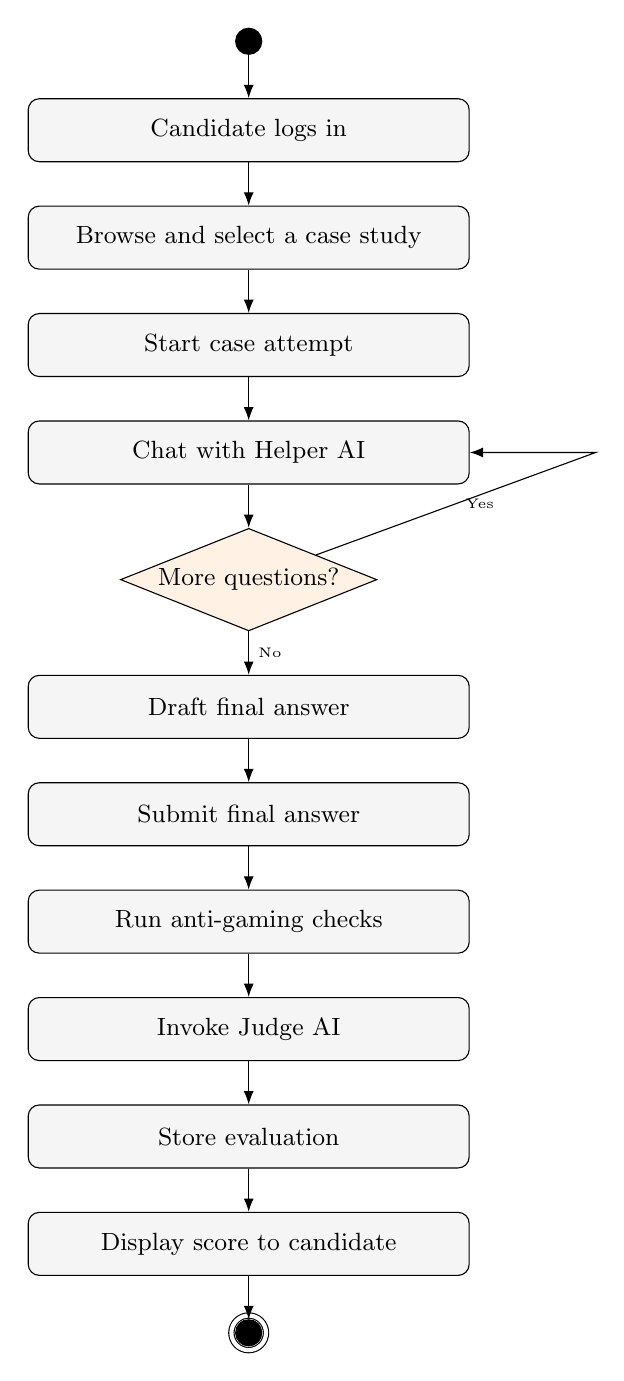
\begin{tikzpicture}[
  act/.style={draw, rounded corners, fill=gray!8, minimum width=5.6cm, minimum height=0.8cm, align=center, font=\small},
  dec/.style={draw, diamond, fill=orange!10, aspect=2.5, align=center, font=\small, inner sep=1pt},
  node distance=0.55cm
]
  \node[circle,draw,fill=black,minimum size=0.25cm] (start) {};
  \node[act, below=of start] (a1) {Candidate logs in};
  \node[act, below=of a1] (a2) {Browse and select a case study};
  \node[act, below=of a2] (a3) {Start case attempt};
  \node[act, below=of a3] (a4) {Chat with Helper AI};
  \node[dec, below=of a4, minimum height=0.9cm] (d1) {More questions?};
  \node[act, below=of d1] (a5) {Draft final answer};
  \node[act, below=of a5] (a6) {Submit final answer};
  \node[act, below=of a6] (a7) {Run anti-gaming checks};
  \node[act, below=of a7] (a8) {Invoke Judge AI};
  \node[act, below=of a8] (a9) {Store evaluation};
  \node[act, below=of a9] (a10) {Display score to candidate};
  \node[circle,draw,fill=black,minimum size=0.25cm, below=of a10] (end) {};
  \draw[double,double distance=1.5pt] (end) circle (0.22cm);

  \draw[-{Latex}] (start) -- (a1);
  \draw[-{Latex}] (a1) -- (a2);
  \draw[-{Latex}] (a2) -- (a3);
  \draw[-{Latex}] (a3) -- (a4);
  \draw[-{Latex}] (a4) -- (d1);
  \draw[-{Latex}] (d1) -- node[right,font=\tiny]{Yes} ($(a4.east)+(1.6,0)$) |- (a4.east);
  \draw[-{Latex}] (d1) -- node[right,font=\tiny]{No} (a5);
  \draw[-{Latex}] (a5) -- (a6);
  \draw[-{Latex}] (a6) -- (a7);
  \draw[-{Latex}] (a7) -- (a8);
  \draw[-{Latex}] (a8) -- (a9);
  \draw[-{Latex}] (a9) -- (a10);
  \draw[-{Latex}] (a10) -- (end);
\end{tikzpicture}
\end{figure}

\newpage
This swimlane diagram illustrates the same workflow split across the Candidate, the Frontend,
the Backend, and the Judge AI, showing where each responsibility sits: the frontend only
relays candidate actions, the backend owns persistence and orchestration, and the Judge AI is
reached only once, at the very end.

\begin{figure}[h]
\centering
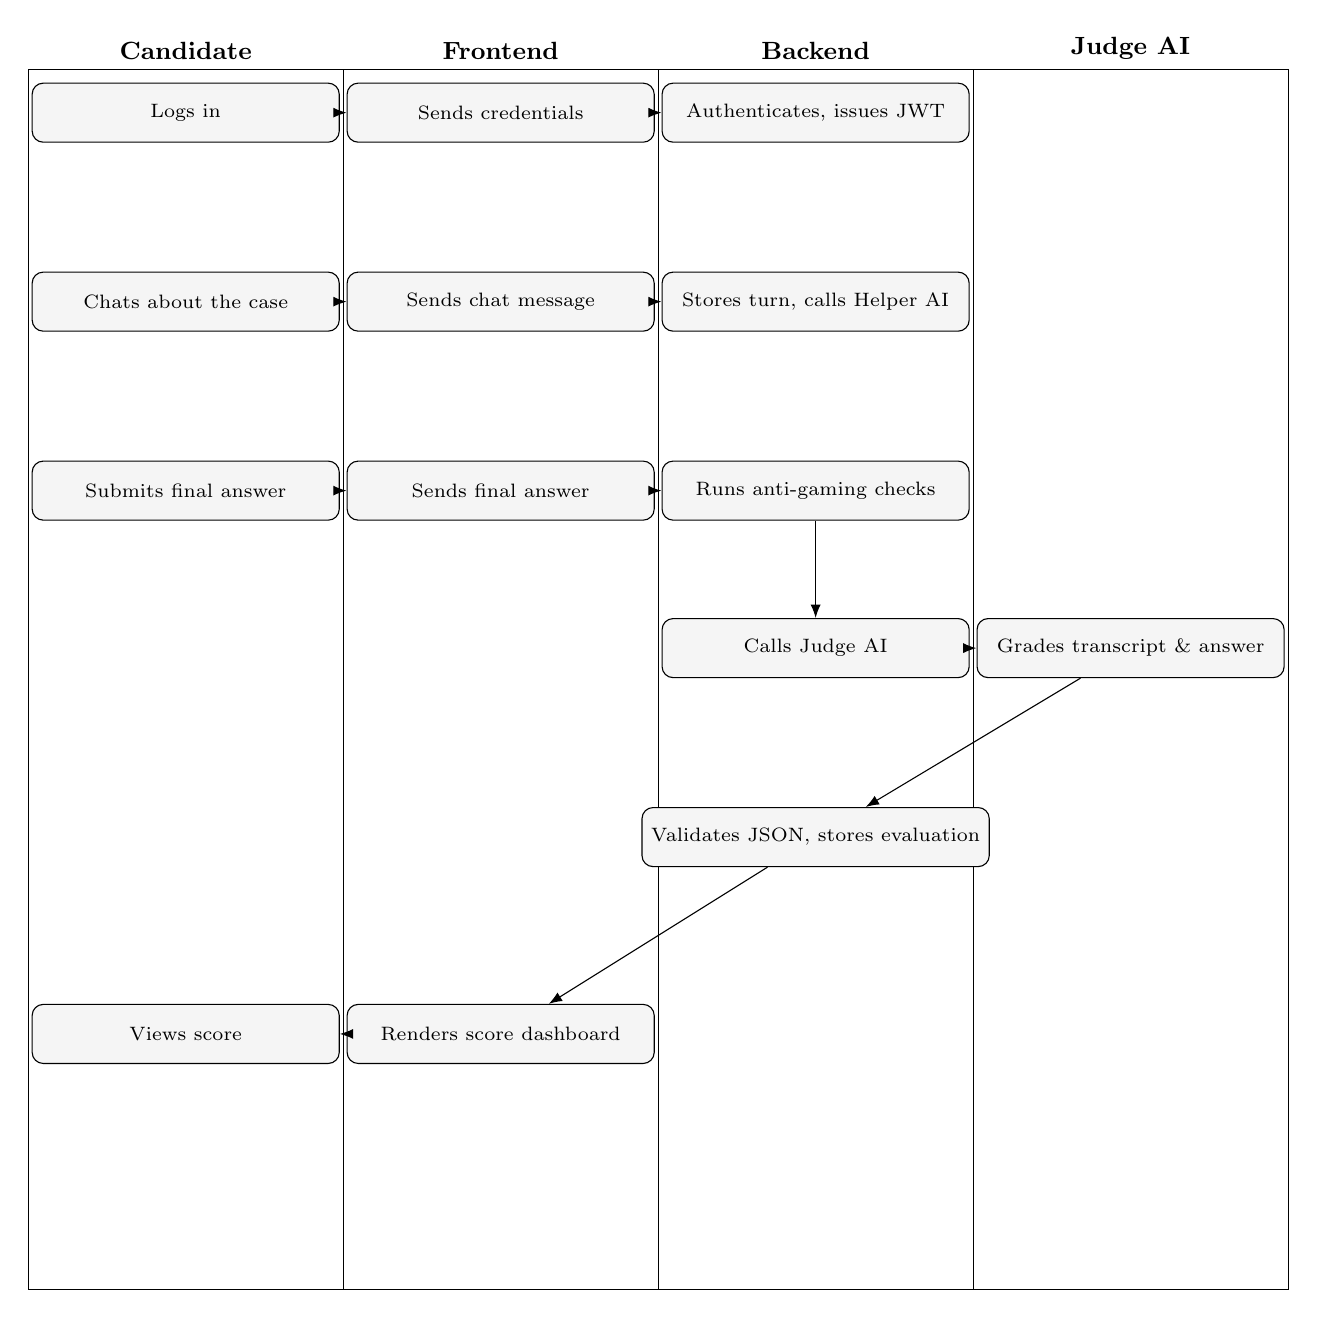
\begin{tikzpicture}[
  act/.style={draw, rounded corners, fill=gray!8, minimum width=3.9cm, minimum height=0.75cm, align=center, font=\scriptsize},
  lane/.style={draw, minimum height=15.5cm}
]
  \node[lane, minimum width=4cm, label={above:\small\bfseries Candidate}] (l1) at (0,0) {};
  \node[lane, minimum width=4cm, label={above:\small\bfseries Frontend}] (l2) at (4,0) {};
  \node[lane, minimum width=4cm, label={above:\small\bfseries Backend}] (l3) at (8,0) {};
  \node[lane, minimum width=4cm, label={above:\small\bfseries Judge AI}] (l4) at (12,0) {};

  \node[act] (c1) at (0,7.2) {Logs in};
  \node[act] (c2) at (0,4.8) {Chats about the case};
  \node[act] (c3) at (0,2.4) {Submits final answer};
  \node[act] (c4) at (0,-4.5) {Views score};

  \node[act] (f1) at (4,7.2) {Sends credentials};
  \node[act] (f2) at (4,4.8) {Sends chat message};
  \node[act] (f3) at (4,2.4) {Sends final answer};
  \node[act] (f4) at (4,-4.5) {Renders score dashboard};

  \node[act] (b1) at (8,7.2) {Authenticates, issues JWT};
  \node[act] (b2) at (8,4.8) {Stores turn, calls Helper AI};
  \node[act] (b3) at (8,2.4) {Runs anti-gaming checks};
  \node[act] (b4) at (8,0.4) {Calls Judge AI};
  \node[act] (b5) at (8,-2.0) {Validates JSON, stores evaluation};

  \node[act] (j1) at (12,0.4) {Grades transcript \& answer};

  \draw[-{Latex}] (c1) -- (f1); \draw[-{Latex}] (f1) -- (b1);
  \draw[-{Latex}] (c2) -- (f2); \draw[-{Latex}] (f2) -- (b2);
  \draw[-{Latex}] (c3) -- (f3); \draw[-{Latex}] (f3) -- (b3);
  \draw[-{Latex}] (b3) -- (b4);
  \draw[-{Latex}] (b4) -- (j1);
  \draw[-{Latex}] (j1) -- (b5);
  \draw[-{Latex}] (b5) -- (f4);
  \draw[-{Latex}] (f4) -- (c4);
\end{tikzpicture}
\end{figure}

\newpage
\subsection{Data Flow Diagrams (DFDs)}
The following figures illustrate the flow of information within PromptBench, from a
high-level context down to detailed process-level data movement.

\subsubsection{DFD Level 0}
This Level 0 diagram provides a high-level overview of the PromptBench system and its
single external entity, the Candidate. The candidate sends chat messages and a final answer,
and receives Helper AI replies and a graded score in return.

\begin{figure}[h]
\centering
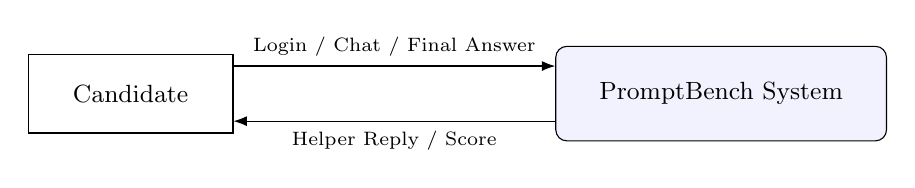
\begin{tikzpicture}[
  ext/.style={draw, minimum width=2.6cm, minimum height=1cm, align=center, font=\small},
  proc/.style={draw, rounded corners, fill=blue!5, minimum width=4.2cm, minimum height=1.2cm, align=center, font=\small}
]
  \node[ext] (cand) at (0,0) {Candidate};
  \node[proc] (sys) at (7.5,0) {PromptBench System};
  \draw[-{Latex}] (cand.east) ++(0,0.35) -- node[above,font=\scriptsize]{Login / Chat / Final Answer} ($(sys.west)+(0,0.35)$);
  \draw[-{Latex}] ($(sys.west)-(0,0.35)$) -- node[below,font=\scriptsize]{Helper Reply / Score} ($(cand.east)-(0,0.35)$);
\end{tikzpicture}
\end{figure}

\subsubsection{DFD Level 1}
This Level 1 diagram breaks the system into its four major processes: Authentication, Case
Management, Submission \& Helper AI Interaction, and Evaluation. Each process reads from
or writes to its corresponding data store.

\begin{figure}[h]
\centering
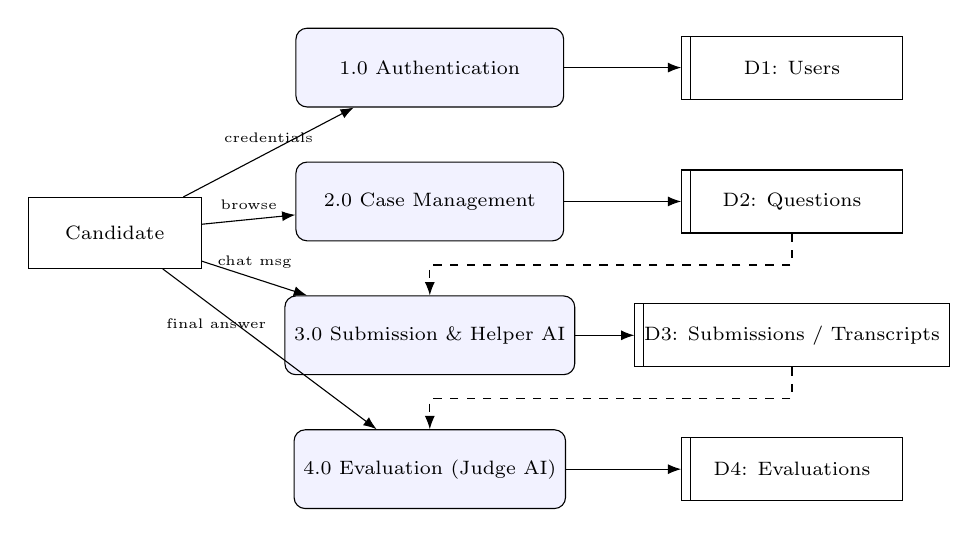
\begin{tikzpicture}[
  ext/.style={draw, minimum width=2.2cm, minimum height=0.9cm, align=center, font=\scriptsize},
  proc/.style={draw, rounded corners, fill=blue!5, minimum width=3.4cm, minimum height=1cm, align=center, font=\scriptsize},
  store/.style={draw, minimum width=2.8cm, minimum height=0.8cm, align=center, font=\scriptsize, path picture={
    \draw ([xshift=3pt]path picture bounding box.north west) -- ([xshift=3pt]path picture bounding box.south west);
  }}
]
  \node[ext] (cand) at (0,3.5) {Candidate};
  \node[proc] (p1) at (4,5.6) {1.0 Authentication};
  \node[proc] (p2) at (4,3.9) {2.0 Case Management};
  \node[proc] (p3) at (4,2.2) {3.0 Submission \& Helper AI};
  \node[proc] (p4) at (4,0.5) {4.0 Evaluation (Judge AI)};

  \node[store] (d1) at (8.6,5.6) {D1: Users};
  \node[store] (d2) at (8.6,3.9) {D2: Questions};
  \node[store] (d3) at (8.6,2.2) {D3: Submissions / Transcripts};
  \node[store] (d4) at (8.6,0.5) {D4: Evaluations};

  \draw[-{Latex}] (cand) -- node[above,font=\tiny]{credentials} (p1);
  \draw[-{Latex}] (cand) -- node[above,font=\tiny]{browse} (p2);
  \draw[-{Latex}] (cand) -- node[above,font=\tiny]{chat msg} (p3);
  \draw[-{Latex}] (cand) -- node[below,font=\tiny,pos=0.25]{final answer} (p4);

  \draw[-{Latex}] (p1) -- (d1);
  \draw[-{Latex}] (p2) -- (d2);
  \draw[-{Latex}] (p3) -- (d3);
  \draw[-{Latex}] (p4) -- (d4);
  \draw[-{Latex}, dashed] (d3.south) -- ++(0,-0.4) -| (p4.north);
  \draw[-{Latex}, dashed] (d2.south) -- ++(0,-0.4) -| (p3.north);
\end{tikzpicture}
\end{figure}

\subsubsection{DFD Level 2}
This Level 2 diagram expands processes 3.0 and 4.0, showing how a chat message becomes a
stored transcript turn and Helper AI reply, and how a final answer flows through anti-gaming
checks and the Judge AI into a stored evaluation.

\begin{figure}[h]
\centering
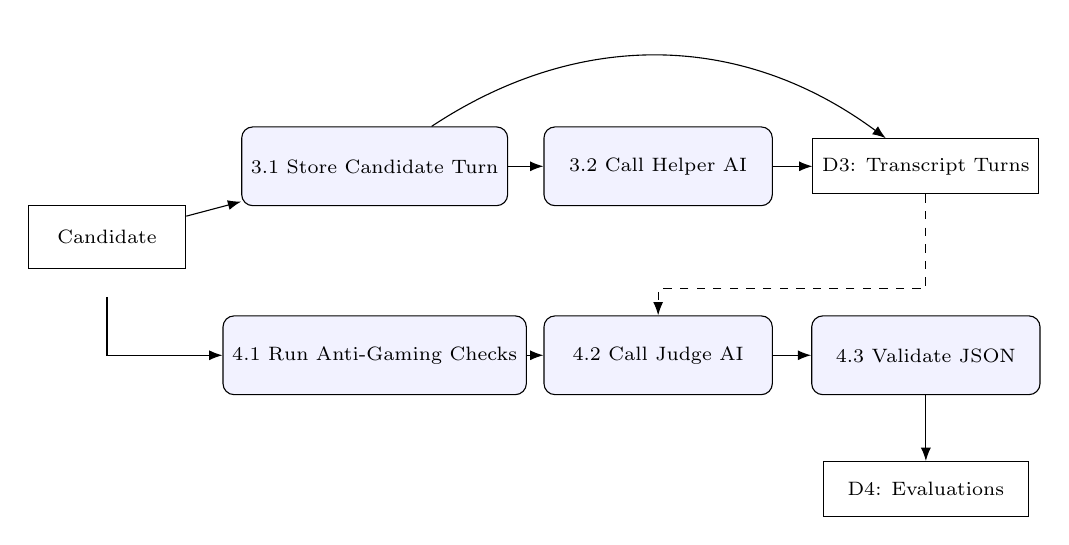
\begin{tikzpicture}[
  ext/.style={draw, minimum width=2cm, minimum height=0.8cm, align=center, font=\scriptsize},
  proc/.style={draw, rounded corners, fill=blue!5, minimum width=2.9cm, minimum height=1cm, align=center, font=\scriptsize},
  store/.style={draw, minimum width=2.6cm, minimum height=0.7cm, align=center, font=\scriptsize}
]
  \node[ext] (cand) at (0,4.5) {Candidate};
  \node[proc] (p31) at (3.4,5.4) {3.1 Store Candidate Turn};
  \node[proc] (p32) at (7,5.4) {3.2 Call Helper AI};
  \node[store] (d3) at (10.4,5.4) {D3: Transcript Turns};

  \node[proc] (p41) at (3.4,3.0) {4.1 Run Anti-Gaming Checks};
  \node[proc] (p42) at (7,3.0) {4.2 Call Judge AI};
  \node[proc] (p43) at (10.4,3.0) {4.3 Validate JSON};
  \node[store] (d4) at (10.4,1.3) {D4: Evaluations};

  \draw[-{Latex}] (cand) -- (p31);
  \draw[-{Latex}] (p31) -- (p32);
  \draw[-{Latex}] (p32) -- (d3);
  \draw[-{Latex}, bend left=35] (p31) to (d3);

  \draw[-{Latex}] ([yshift=-10pt]cand.south) |- (p41);
  \draw[-{Latex}] (p41) -- (p42);
  \draw[-{Latex}] (p42) -- (p43);
  \draw[-{Latex}] (p43) -- (d4);
  \draw[-{Latex}, dashed] (d3.south) -- ++(0,-1.2) -| (p42.north);
\end{tikzpicture}
\end{figure}

\newpage
\subsection{Software Requirement Specification (IEEE Format)}
\textbf{PromptBench}

\subsubsection{Introduction}
\textbf{Purpose}\\
The purpose of this document is to provide a detailed description of the PromptBench
system, a platform designed to let candidates practice and be evaluated on their ability to
solve open-ended business problems in collaboration with an AI assistant. This document
serves as a reference for developers (system design and implementation), instructors
(evaluation criteria), and candidates (end users).

\textbf{Scope}\\
PromptBench is a web-based system that:
\begin{itemize}[nosep]
  \item Presents business case studies across three categories: data diagnosis, strategy generation, and customer reasoning.
  \item Provides a Helper AI for candidates to converse with while investigating a case.
  \item Grades the full transcript and final answer using a private Judge AI against a hidden rubric and ground truth.
  \item Flags likely attempts to game the assessment.
\end{itemize}

\textbf{Definitions, Acronyms, Abbreviations}
\begin{itemize}[nosep]
  \item \textbf{Helper AI:} candidate-facing assistant with access only to public case context.
  \item \textbf{Judge AI:} server-side evaluator with access to the rubric and ground truth.
  \item \textbf{Rubric:} weighted scoring dimensions used by the Judge AI.
  \item \textbf{Ground truth notes:} hidden reference notes never shown to the candidate or Helper AI.
  \item \textbf{JWT:} JSON Web Token, used for authenticating API requests.
  \item \textbf{DB:} Database.
\end{itemize}

\textbf{References}
\begin{itemize}[nosep]
  \item IEEE SRS Standards.
  \item Software Engineering course material.
\end{itemize}

\textbf{Overview}\\
This document describes system features, functional and non-functional requirements, user
roles, and system constraints.

\subsubsection{Overall Description}
\textbf{Product Perspective}\\
PromptBench is a standalone web application consisting of a React frontend, a FastAPI
backend, a PostgreSQL database, and an external AI provider (Claude API) used for both the
Helper AI and Judge AI roles.

\textbf{Product Functions}\\
Candidate functions: sign up / log in, browse case studies, start an attempt, chat with the
Helper AI, submit a final answer, view evaluation score, view attempt history.\\
System functions: generate Helper AI responses, run anti-gaming checks, grade submissions
via the Judge AI.

\textbf{User Characteristics}
\begin{itemize}[nosep]
  \item \textbf{Candidate:} basic technical/business literacy, uses the system to practice a skill.
  \item \textbf{Helper AI / Judge AI:} automated system actors, no human interaction.
\end{itemize}

\textbf{Constraints}
\begin{itemize}[nosep]
  \item Requires an internet connection and a configured Claude API key.
  \item Currently targets local development; no deployment configuration exists yet.
\end{itemize}

\textbf{Assumptions and Dependencies}
\begin{itemize}[nosep]
  \item Users have basic digital literacy.
  \item The Claude API is available and returns well-formed responses (or the system falls back to mocked responses in test mode).
\end{itemize}

\subsubsection{Specific Requirements}
\textbf{External Interface Requirements}\\
User Interface: simple login/signup forms, a case list, a chat-style case workspace, and a
score dashboard.\\
Software Interface: PostgreSQL database, Anthropic Claude API.

\textbf{Functional Requirements}
\begin{description}[nosep]
  \item[FR1 -- Sign Up / Log In:] Input: email, password (+ name). Output: account created / JWT issued.
  \item[FR2 -- List Case Studies:] Output: list of questions with title, category, difficulty.
  \item[FR3 -- Start Submission:] Input: question id. Output: new submission id.
  \item[FR4 -- Send Chat Message:] Input: message text. Output: Helper AI reply, persisted transcript turn.
  \item[FR5 -- Submit Final Answer:] Input: final answer text. Output: structured evaluation (overall score, dimension scores, reasoning).
  \item[FR6 -- Run Anti-Gaming Checks:] Output: list of warning flags attached to the evaluation.
  \item[FR7 -- View Evaluation:] Output: full evaluation report and transcript for a submission.
  \item[FR8 -- View Attempt History:] Output: list of past graded submissions and scores.
\end{description}

\textbf{Performance Requirements}
\begin{itemize}[nosep]
  \item API responses (excluding LLM calls) should return in under 1 second under normal load.
  \item The system should support multiple concurrent candidates without cross-contaminating sessions.
\end{itemize}

\textbf{Logical Database Requirements}\\
The system includes five entities: User, Question, Submission, TranscriptTurn, and
Evaluation (see the Entity-Relationship Diagram in Section 2.6). Each entity has a unique
identifier and well-defined relationships with the others.

\textbf{Quality Attributes}
\begin{itemize}[nosep]
  \item \textbf{Usability:} simple, chat-first workspace.
  \item \textbf{Reliability:} retry-safe JSON parsing for the Judge AI's structured output.
  \item \textbf{Scalability:} stateless JWT auth allows horizontal scaling of the backend.
  \item \textbf{Security:} bcrypt password hashing, JWT-protected routes, strict ownership checks on every submission and evaluation endpoint.
  \item \textbf{Integrity:} architectural isolation between the Helper AI and Judge AI.
\end{itemize}

\textbf{Other Requirements}\\
\textit{Future Enhancements:} configurable rubric schemas per category, an admin interface for
authoring case studies, deployment to a cloud platform, and score-weighted anti-gaming
penalties.

\newpage
\subsection{User Stories and User Cards}

\textbf{User Stories -- PromptBench}
\begin{enumerate}[nosep]
  \item As a candidate, I want to browse business case studies so that I can choose one to practice.
  \item As a candidate, I want to chat with a Helper AI so that I can investigate the case before answering.
  \item As a candidate, I want to submit a final recommendation so that my work can be graded.
  \item As a candidate, I want to see a per-dimension score breakdown so that I understand exactly where I did well or fell short.
  \item As a candidate, I want to review my past attempts so that I can track my improvement over time.
  \item As the Judge AI, I need the rubric and hidden ground truth so that I can grade objectively without ever exposing them to the candidate.
  \item As the system, I want to flag near-zero-effort or pre-written submissions so that the evaluation stays meaningful.
\end{enumerate}

\textbf{Story Cards}

\noindent\rule{\linewidth}{0.5pt}\\
\textbf{Story Card 1}\\
\textbf{Title:} Browse Case Studies\\
\textbf{Actor:} Candidate\\
\textbf{Description:} Candidate views the list of available case studies.\\
\textbf{Acceptance Criteria:}
\begin{itemize}[nosep]
  \item System displays title, category, and difficulty for each case.
  \item Hidden fields (rubric, ground truth) are never included in the response.
\end{itemize}

\noindent\rule{\linewidth}{0.5pt}\\
\textbf{Story Card 2}\\
\textbf{Title:} Chat with Helper AI\\
\textbf{Actor:} Candidate\\
\textbf{Description:} Candidate exchanges messages with the Helper AI.\\
\textbf{Acceptance Criteria:}
\begin{itemize}[nosep]
  \item Every message and reply is persisted in order.
  \item The Helper AI only receives the public case context, never the rubric.
\end{itemize}

\noindent\rule{\linewidth}{0.5pt}\\
\textbf{Story Card 3}\\
\textbf{Title:} Submit Final Answer\\
\textbf{Actor:} Candidate\\
\textbf{Description:} Candidate submits their final recommendation for grading.\\
\textbf{Acceptance Criteria:}
\begin{itemize}[nosep]
  \item Anti-gaming checks run automatically at submission time.
  \item The Judge AI's structured response is validated before being stored.
\end{itemize}

\noindent\rule{\linewidth}{0.5pt}\\
\textbf{Story Card 4}\\
\textbf{Title:} View Evaluation Score\\
\textbf{Actor:} Candidate\\
\textbf{Description:} Candidate reviews the graded result of a submission.\\
\textbf{Acceptance Criteria:}
\begin{itemize}[nosep]
  \item Overall score, dimension scores, reasoning, and any anti-gaming flags are shown.
  \item Only the owning candidate can view the evaluation.
\end{itemize}

\noindent\rule{\linewidth}{0.5pt}\\
\textbf{Story Card 5}\\
\textbf{Title:} View Attempt History\\
\textbf{Actor:} Candidate\\
\textbf{Description:} Candidate views a history of past graded attempts.\\
\textbf{Acceptance Criteria:}
\begin{itemize}[nosep]
  \item List is ordered by most recent submission first.
  \item Only \texttt{submitted} (fully graded) attempts are shown.
\end{itemize}

\noindent\rule{\linewidth}{0.5pt}\\
\textbf{Story Card 6}\\
\textbf{Title:} Grade Submission\\
\textbf{Actor:} Judge AI\\
\textbf{Description:} System grades the transcript and final answer against a hidden rubric.\\
\textbf{Acceptance Criteria:}
\begin{itemize}[nosep]
  \item Returned JSON is validated against a strict schema before being stored.
  \item On failure, the submission is marked \texttt{evaluation\_failed} and can be retried.
\end{itemize}

\noindent\rule{\linewidth}{0.5pt}\\
\textbf{Story Card 7}\\
\textbf{Title:} Run Anti-Gaming Checks\\
\textbf{Actor:} System\\
\textbf{Description:} System flags submissions that show signs of gaming the assessment.\\
\textbf{Acceptance Criteria:}
\begin{itemize}[nosep]
  \item Near-zero conversation, too-fast submission, and pre-written-answer patterns are each independently detected.
  \item Flags are stored alongside the evaluation, not used to block submission.
\end{itemize}

\subsection{Entity-Relationship Diagram}

The Entity-Relationship diagram of the PromptBench system captures its five core entities --
\texttt{USER}, \texttt{QUESTION}, \texttt{SUBMISSION}, \texttt{TRANSCRIPT\_TURN}, and
\texttt{EVALUATION} -- along with an embedded \texttt{DIMENSION\_SCORES} structure. A
\texttt{USER} creates many \texttt{SUBMISSION}s, and each \texttt{SUBMISSION} is tied to
one \texttt{QUESTION}. A \texttt{SUBMISSION} in turn contains many
\texttt{TRANSCRIPT\_TURN} records (the full chat history) and is evaluated by exactly one
\texttt{EVALUATION}, which embeds the four rubric dimension scores produced by the Judge
AI. This structure directly mirrors the SQLAlchemy models used in the backend.

\begin{figure}[p]
\centering
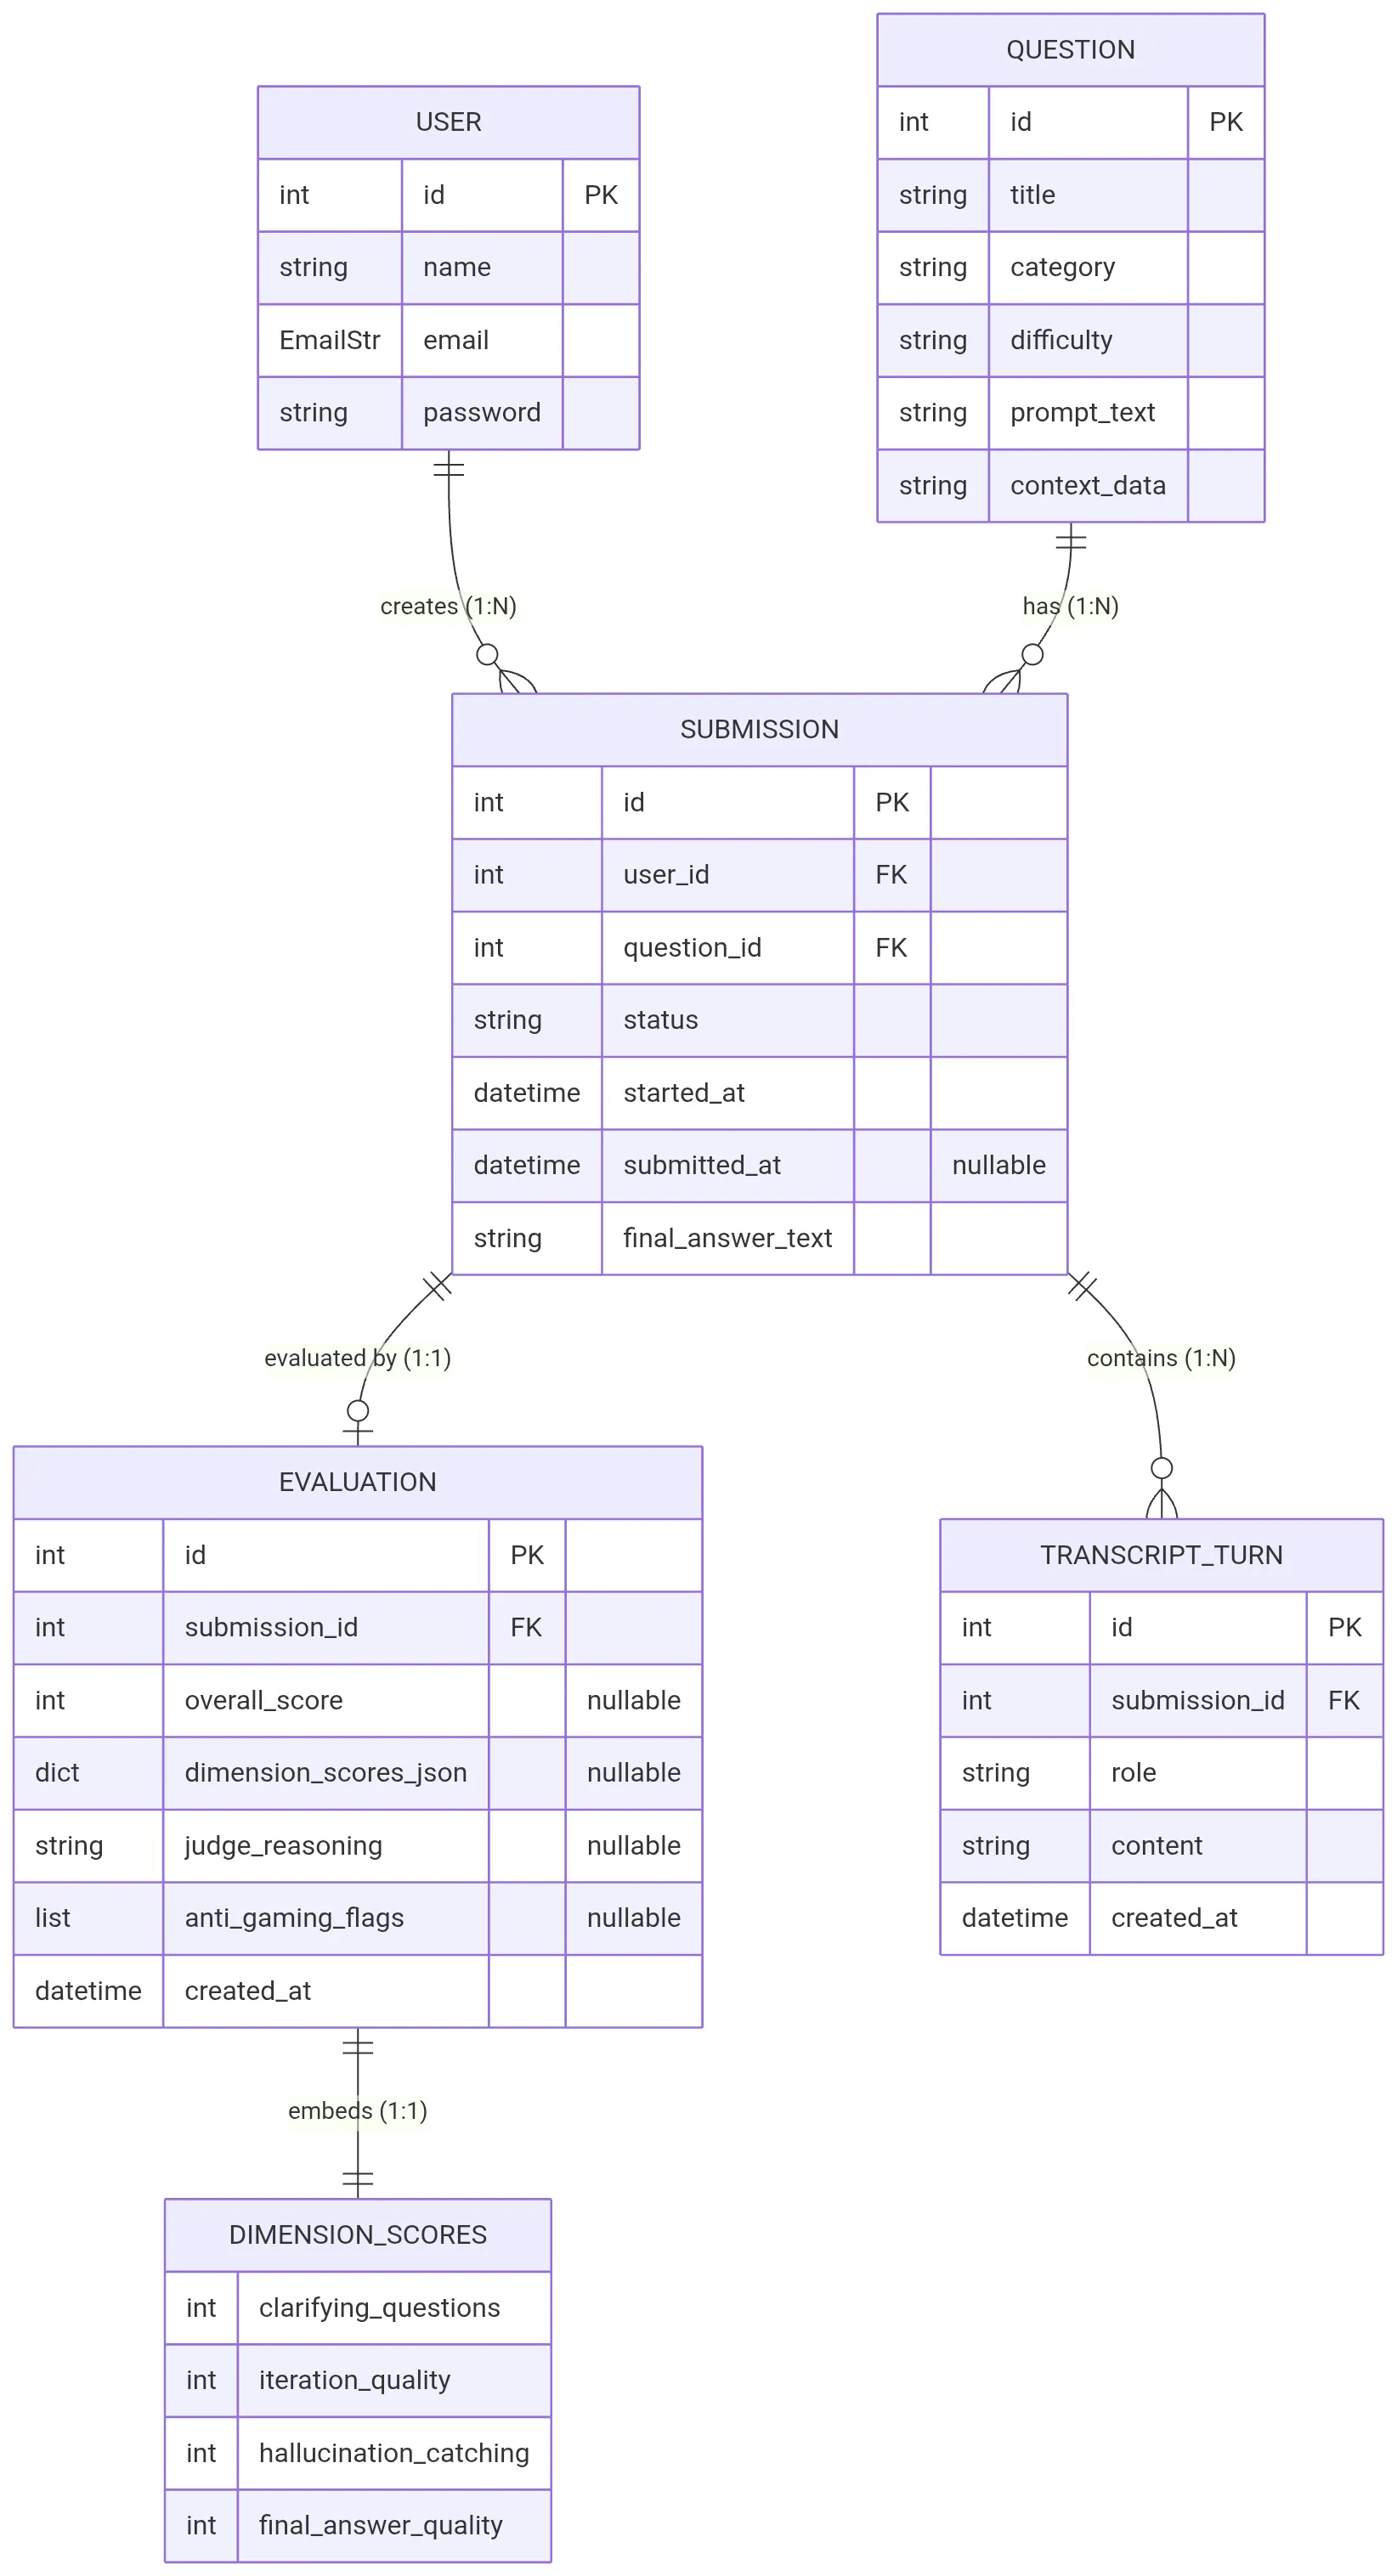
\includegraphics[height=0.88\textheight,keepaspectratio]{images/er_diagram_light.png}
\caption{Entity-Relationship Diagram -- PromptBench}
\end{figure}

\subsection{Class Diagram}

The class diagram of the PromptBench system represents its static structure: the persistent
domain classes (User, Question, Submission, TranscriptTurn, Evaluation) alongside the three
service-level classes that implement the system's core behaviour (HelperAIService,
JudgeAIService, AntiGamingChecker). The service classes operate on domain objects but are
not themselves persisted.

\begin{figure}[h]
\centering
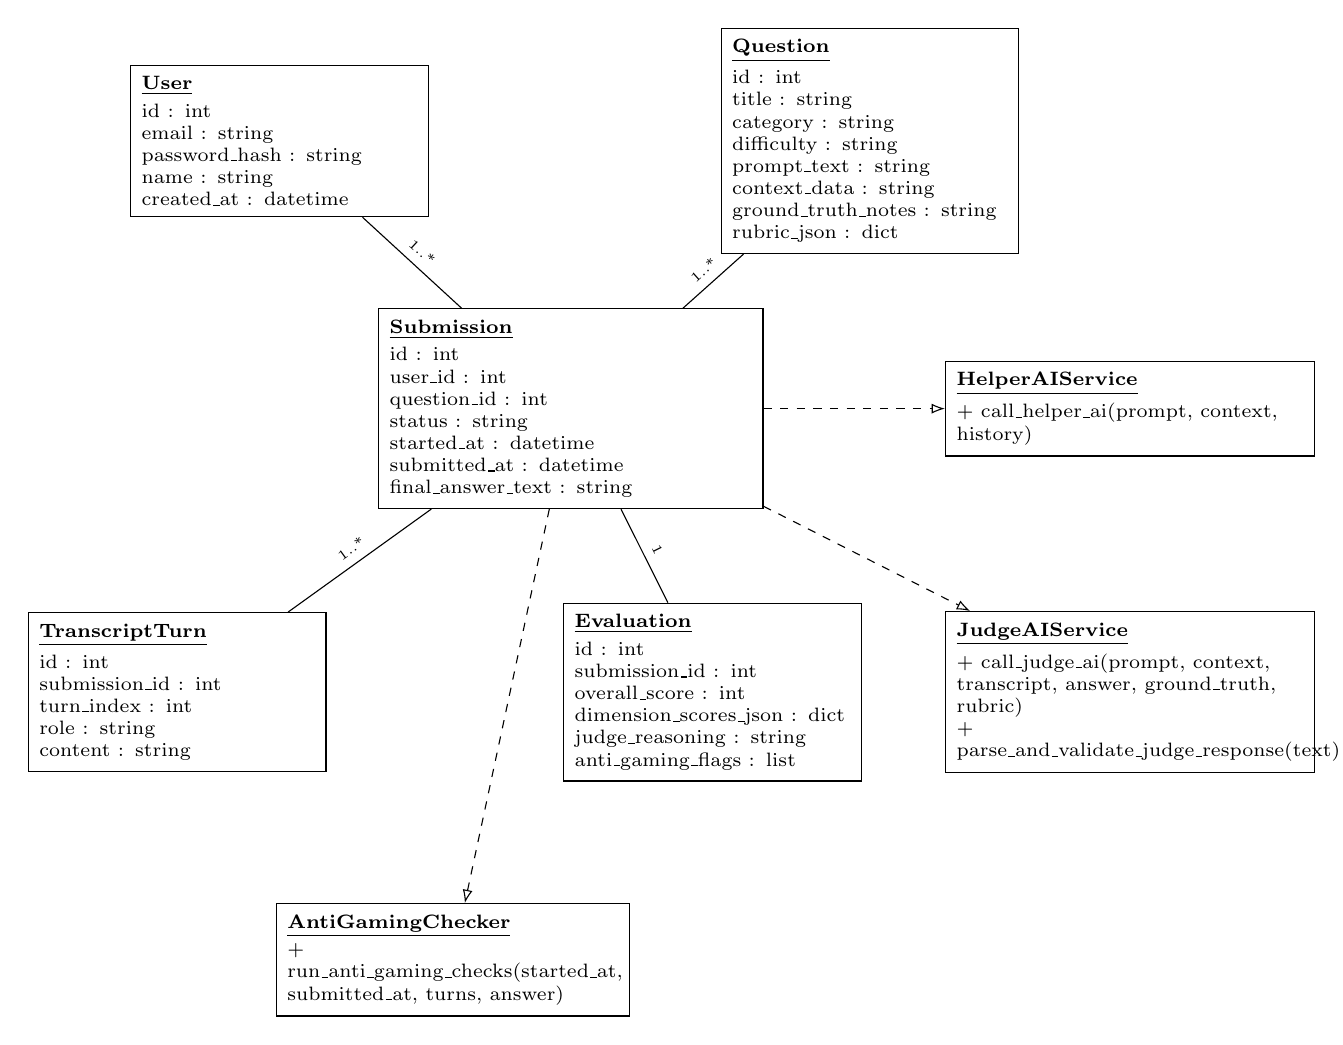
\begin{tikzpicture}[
  cls/.style={draw, rectangle, align=left, font=\scriptsize, text width=3.5cm, inner sep=4pt},
  every node/.style={font=\scriptsize}
]
  \node[cls] (user) at (0,7) {
    \underline{\textbf{User}}\\[2pt]
    id : int\\ email : string\\ password\_hash : string\\ name : string\\ created\_at : datetime
  };
  \node[cls] (question) at (7.5,7) {
    \underline{\textbf{Question}}\\[2pt]
    id : int\\ title : string\\ category : string\\ difficulty : string\\ prompt\_text : string\\ context\_data : string\\ ground\_truth\_notes : string\\ rubric\_json : dict
  };
  \node[cls, text width=4.6cm] (submission) at (3.7,3.6) {
    \underline{\textbf{Submission}}\\[2pt]
    id : int\\ user\_id : int\\ question\_id : int\\ status : string\\ started\_at : datetime\\ submitted\_at : datetime\\ final\_answer\_text : string
  };
  \node[cls] (turn) at (-1.3,0) {
    \underline{\textbf{TranscriptTurn}}\\[2pt]
    id : int\\ submission\_id : int\\ turn\_index : int\\ role : string\\ content : string
  };
  \node[cls] (eval) at (5.5,0) {
    \underline{\textbf{Evaluation}}\\[2pt]
    id : int\\ submission\_id : int\\ overall\_score : int\\ dimension\_scores\_json : dict\\ judge\_reasoning : string\\ anti\_gaming\_flags : list
  };
  \node[cls, text width=4.4cm] (helper) at (10.8,3.6) {
    \underline{\textbf{HelperAIService}}\\[2pt]
    + call\_helper\_ai(prompt, context, history)
  };
  \node[cls, text width=4.4cm] (judge) at (10.8,0) {
    \underline{\textbf{JudgeAIService}}\\[2pt]
    + call\_judge\_ai(prompt, context, transcript, answer, ground\_truth, rubric)\\
    + parse\_and\_validate\_judge\_response(text)
  };
  \node[cls, text width=4.2cm] (anti) at (2.2,-3.4) {
    \underline{\textbf{AntiGamingChecker}}\\[2pt]
    + run\_anti\_gaming\_checks(started\_at, submitted\_at, turns, answer)
  };

  \draw (user) -- node[above,sloped,font=\tiny]{1..*} (submission);
  \draw (question) -- node[above,sloped,font=\tiny]{1..*} (submission);
  \draw (submission) -- node[above,sloped,font=\tiny]{1..*} (turn);
  \draw (submission) -- node[above,sloped,font=\tiny]{1} (eval);
  \draw[dashed,-{Latex[open]}] (submission) -- (helper);
  \draw[dashed,-{Latex[open]}] (submission) -- (judge);
  \draw[dashed,-{Latex[open]}] (submission) -- (anti);
\end{tikzpicture}
\end{figure}

\end{document}
